% TAME: Transfer-Aware Model-Harness Co-Evolution through Learned Harness Revisions
% Figure 2 (Overview of TAME) of the paper, re-laid out into three columns so it fills a 16:10
% thumbnail. Adapted from the paper source (tame_iclr2027.tex): same nodes, labels, arrow styles,
% colors and fonts.
\documentclass[tikz,border=1pt]{standalone}
\usepackage{times}
\usepackage{amsmath,amssymb}
\usetikzlibrary{arrows.meta,backgrounds,calc,positioning,shapes.geometric}
\definecolor{tameteal}{HTML}{178A83}
\definecolor{tametealfill}{HTML}{E2F5F2}
\definecolor{tameorange}{HTML}{D47A1F}
\definecolor{tameorangefill}{HTML}{FFF0DD}
\definecolor{tamepurple}{HTML}{7556A5}
\definecolor{tamepurplefill}{HTML}{F0E9FA}
\definecolor{tamegray}{HTML}{59636E}
\definecolor{tamegrayfill}{HTML}{F2F4F6}
\newcommand{\MetaTrain}{\mathcal D_{\mathrm{meta}}}
\newcommand{\Tscore}{\mathcal T}
\newcommand{\Escore}{\mathcal H_{\mathrm{score}}}
\tikzset{flow/.style={-{Latex[length=1.8mm]},thick,draw=tamegray}}
\begin{document}
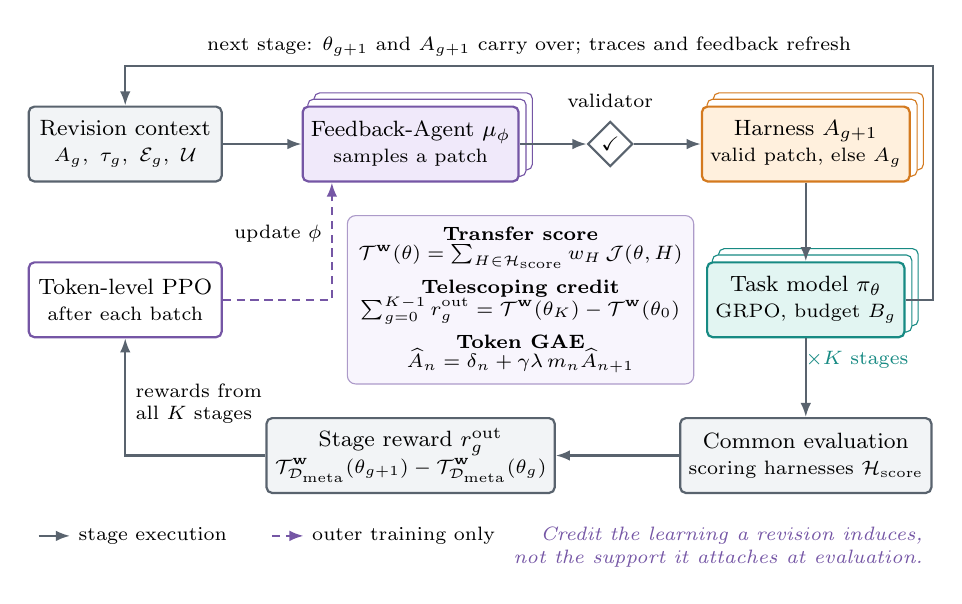
\begin{tikzpicture}[
  stage/.style={draw=tamegray,fill=tamegrayfill,rounded corners=2pt,thick,align=center,
    inner sep=3pt,font=\footnotesize,minimum width=2.45cm,minimum height=0.95cm},
  sub/.style={font=\scriptsize},
  update/.style={-{Latex[length=1.8mm]},thick,draw=tamepurple,densely dashed},
  stack/.style={draw=#1,fill=white,rounded corners=2pt,thin}]
% Row 1: revision context -> Feedback-Agent -> validator -> harness.
\node[stage] (ctx) {Revision context\\{\scriptsize$A_g,\ \tau_g,\ \mathcal E_g,\ \mathcal U$}};
\node[stage,draw=tamepurple,fill=tamepurplefill,right=1.0cm of ctx] (fa) {Feedback-Agent $\mu_\phi$\\{\scriptsize samples a patch}};
\node[stage,draw=tameorange,fill=tameorangefill,right=2.3cm of fa] (h) {Harness $A_{g+1}$\\{\scriptsize valid patch, else $A_g$}};
\node[diamond,draw=tamegray,fill=white,thick,inner sep=1.2pt,font=\scriptsize] (val) at ($(fa.east)!0.5!(h.west)$) {$\checkmark$};
\node[sub,above=1pt of val] {validator};
% Right column going down: task model -> common evaluation.
\node[stage,draw=tameteal,fill=tametealfill,below=1.0cm of h] (tm) {Task model $\pi_\theta$\\{\scriptsize GRPO, budget $B_g$}};
\node[stage,below=1.0cm of tm] (ev) {Common evaluation\\{\scriptsize scoring harnesses $\Escore$}};
% Middle column: stage reward; left column: token-level PPO.
\node[stage] (rw) at (fa |- ev)
  {Stage reward $r_g^{\mathrm{out}}$\\{\scriptsize$\Tscore_{\MetaTrain}^{\mathbf w}(\theta_{g+1})-\Tscore_{\MetaTrain}^{\mathbf w}(\theta_g)$}};
\node[stage,draw=tamepurple,fill=white] (ppo) at (ctx |- tm) {Token-level PPO\\{\scriptsize after each batch}};
% K stages: stacked copies behind the per-stage boxes.
\begin{scope}[on background layer]
  \foreach \n/\c in {fa/tamepurple,h/tameorange,tm/tameteal} {
    \draw[stack=\c] ($(\n.south west)+(0.16,0.16)$) rectangle ($(\n.north east)+(0.16,0.16)$);
    \draw[stack=\c] ($(\n.south west)+(0.08,0.08)$) rectangle ($(\n.north east)+(0.08,0.08)$);
  }
\end{scope}
\node[sub,anchor=north east,text=tameteal] at ($(tm.south east)+(0.16,-0.04)$) {$\times K$ stages};
% Arrows.
\draw[flow] (ctx) -- (fa);
\draw[flow] (fa) -- (val);
\draw[flow] (val) -- (h);
\draw[flow] (h) -- (tm);
\draw[flow] (tm) -- (ev);
\draw[flow] (ev) -- (rw);
\draw[flow] (rw.west) -| node[pos=0.72,right,sub,align=left] {rewards from\\all $K$ stages} (ppo.south);
\draw[update] (ppo.east) -| node[pos=0.78,left,sub] {update $\phi$} ([xshift=-1.0cm]fa.south);
% Next stage: loop from the task model back to the revision context over the top.
\draw[flow] (tm.east) -- ++(0.35,0) |- ($(ctx.north)+(0,0.5)$) node[pos=0.75,above,sub,align=center]
  {next stage: $\theta_{g+1}$ and $A_{g+1}$ carry over; traces and feedback refresh} -- (ctx.north);
% Key quantities (Section 4 of the paper).
\node[draw=tamepurple!60,fill=tamepurplefill!45,rounded corners=3pt,thin,align=center,inner sep=4pt,
      font=\scriptsize] (eqs)
  at ($([xshift=-1.0cm]fa.south |- tm)!0.5!(tm.west)+(0.02,0)$)
  {\textbf{Transfer score}\\[-1pt]
   \mbox{$\Tscore^{\mathbf w}(\theta)=\sum_{H\in\Escore} w_H\,\mathcal J(\theta,H)$}\\[3pt]
   \textbf{Telescoping credit}\\[-1pt]
   \mbox{$\sum_{g=0}^{K-1} r_g^{\mathrm{out}}=\Tscore^{\mathbf w}(\theta_K)-\Tscore^{\mathbf w}(\theta_0)$}\\[3pt]
   \textbf{Token GAE}\\[-1pt]
   \mbox{$\widehat A_n=\delta_n+\gamma\lambda\, m_n\widehat A_{n+1}$}};
% Legend and the paper's key insight.
\node[sub,anchor=north west] (leg) at ($(ctx.west |- rw.south)+(0,-0.3)$)
  {\tikz[baseline=-0.6ex]\draw[flow] (0,0) -- (0.4,0);\ stage execution\qquad
   \tikz[baseline=-0.6ex]\draw[update] (0,0) -- (0.4,0);\ outer training only};
\node[sub,anchor=north east,align=right,text=tamepurple] at ($(ev.east |- rw.south)+(0,-0.3)$)
  {\textit{Credit the learning a revision induces,}\\\textit{not the support it attaches at evaluation.}};
\end{tikzpicture}
\end{document}
